\documentclass{masterthesis}

\usepackage{hyperref} % links
\usepackage{graphicx}
\usepackage{amsmath}
\usepackage{amssymb}
\usepackage{qcircuit}
\usepackage{braket}
\usepackage{float}
\usepackage[toc,page]{appendix}

\begin{document}

\title{Mathematical Modeling of Quantum Repeaters Chains}

\author{Lorenzo La Corte}

\advisor{}

\examiner{}

\maketitle

\chapter*{Mathematical Background}

\section*{Convolution}

Convolution is a fundamental mathematical operation used to combine two functions to produce a third function, which represents how the shape of one function is modified by the other. 

For two discrete functions \(a\) and \(b\), the convolution \(a * b\) is defined as:

\begin{equation}
    (a * b)(z) = \sum_{x=0}^{z} a(x) \cdot b(z - x)
\end{equation}

\paragraph*{Convolution of two Probability Distributions}
In the context of probability distributions, if \(X\) and \(Y\) are independent random variables with probability distribution functions \(p_X\) and \(p_Y\), their sum \(Z = X + Y\) has a probability distribution function \(p_Z\) given by the convolution of \(p_X\) and \(p_Y\):
\begin{equation}\label{eq:convolution}
    p_Z(z) = \sum_{x=0}^{z} p_X(x) \cdot p_Y(z - x)
\end{equation}

Thus, convolution is used to determine the probability distribution of the sum of independent random variables by combining their individual probability distributions.

\paragraph*{Example} 

Consider this simple example. Let $X$ and $Y$ discrete independent random variables. 

The probability distribution $\Pr(Z = z)$ of the random variable $Z = X + Y$ is computed as follows:
\begin{equation}
    \begin{array}{|c|c|c|c|c|c|c|}
        \hline
        x & \Pr(X = x) & y & \Pr(Y = y) & z & \Pr(Z = z) & \text{Derivation of }\Pr(Z = z)\\
        \hline
        0 & 0.2 & 0 & 0.3 & 0 & 0.06 & 0.2 \cdot 0.3 \\
        \hline
        1 & 0.5 & 1 & 0.4 & 1 & 0.23 & 0.2 \cdot 0.4 + 0.5 \cdot 0.3 \\
        \hline
        2 & 0.3 & 2 & 0.3 & 2 & 0.35 & 0.2 \cdot 0.3 + 0.5 \cdot 0.4 + 0.3 \cdot 0.3 \\
        \hline
         &  &  &  & 3 & 0.27 & 0.5 \cdot 0.3 + 0.3 \cdot 0.4 \\
        \hline
         &  &  &  & 4 & 0.09 & 0.3 \cdot 0.3 \\
        \hline
    \end{array}
\end{equation}

Note that $\Pr(Z = z)$ has five elements (all the possible sums), and it is valid as its probabilities sum to 1.

\begin{samepage}\label{page:convolution_associativity}
    The convolution operator \( * \) is associative, meaning that for any three functions \(a\), \(b\), and \(c\):
    \begin{equation}
        (a * b) * c = a * (b * c)
    \end{equation}        
\end{samepage}

\section*{Random Variables}

In this section, we fix notation on random variables and operations on them. 

Most random variables in the context of quantum repeaters
\begin{itemize}
    \item are discrete,
    \item have as domain a subset of nonnegative integers.
\end{itemize}

\paragraph*{PDF}\label{paragraph:pdf}
Let $X$ be such a random variable, then its probability distribution function is a map
\begin{equation}
    p_X : x \mapsto \Pr(X = x)
\end{equation} 
which describes the probability that its outcome will be $x \in \{0, 1, 2, \ldots \}$.

\paragraph*{CDF}\label{paragraph:cdf}
Equivalently, $X$ is described by its cumulative distribution function
\begin{equation}
    \Pr(X \leq x) = \sum_{y=0}^{x} \Pr(X = y),
\end{equation}

which is transformed to the probability distribution function as 
\begin{equation}
    \Pr(X = x) = \Pr(X \leq x) - \Pr(X \leq x - 1).
\end{equation}

\paragraph*{Independent Random Variables}\label{paragraph:independent_random_variables}
Two random variables $X$ and $Y$ are independent if 
\begin{equation}
    \Pr(X = x \text{ and } Y = y) = \Pr(X = x) \cdot \Pr(Y = y)
\end{equation}
for all $x$ and $y$ in the domain.

\paragraph*{Copies of a Random Variable}\label{paragraph:copies_of_a_random_variable}
By a \textit{copy} of $X$, we mean a fresh random variable which is independent from $X$ and identically distributed (i.i.d.).
We will denote a copy by a superscript in parentheses. For example, $X^{(1)}$, $X^{(142)}$ and $X^{(A)}$ are all copies of $X$.

The mean of $X$ is denoted by 
\begin{equation}\label{eq:expectation}
    E[X] = \sum_{x=0}^{\infty} \Pr(X = x) \cdot x
\end{equation}

and can equivalently be computed as 
\begin{equation}
    E[X] = \sum_{x=1}^{\infty} \Pr(X \geq x).
\end{equation}

\paragraph*{Function of Random Variables}\label{paragraph:function_of_random_variables}
If $f$ is a function which takes two nonnegative integers as input, then the random variable $f(X, Y)$ has probability distribution function defined as

\begin{equation}
    \Pr(f(X, Y) = z) := \sum_{\substack{x=0, y=0 \\ f(x,y)=z}}^{\infty} \Pr(X = x \text{ and } Y = y).
\end{equation}

\paragraph*{Sum of Random Variables}\label{paragraph:sum_of_random_variables}
An example of such a function is addition. 

Define $Z := X+Y$ where $X$ and $Y$ are independent, then the probability distribution $p_Z$ of $Z$ is given by 
\begin{equation}
    p_Z(z) = \Pr(Z = z) = \sum_{\substack{x=0, y=0 \\ x+y=z}}^{\infty} \Pr(X = x \text{ and } Y = y).
\end{equation}

But since $y = z - x$ this is equivalent to
\begin{align}
    p_Z(z) = \Pr(Z = z) &= \sum_{\substack{x=0}}^{z} \Pr(X = x \text{ and } Y = z - x) \\ 
                        &= \sum_{\substack{x=0}}^{z} \Pr(X = x) \cdot Pr(Y = z - x) \\
                        &= \sum_{x=0}^{z} p_X(x) \cdot p_Y (z - x)
\end{align}
which is the convolution of the distributions $p_X$ and $p_Y$, denoted as $p_Z = p_X * p_Y$ \hyperref[eq:convolution]{(see convolution)}.

Since convolution operator $*$ is associative, writing $a * b * c$ is well-defined, for functions $a$, $b$, $c$ from the nonnegative integers to the real numbers \hyperref[page:convolution_associativity]{(see associativity of convolution)}.
In general, \textbf{the probability distribution of sums of independent random variables equals the convolutions of their individual probability distribution functions}.

\section*{Geometric Distribution}\label{section:geometric_distribution}

The Geometric Distribution is a discrete probability distribution that models the number of trials needed to achieve the first success in a sequence of independent Bernoulli trials, each with the same success probability \( p \).

\subsection*{Probability Distribution Function (PDF)}\label{subsection:geometric_pdf}

The Probability Distribution Function (PDF) of a Geometric Distribution gives the probability that the first success occurs on the \( t \)-th trial. It is defined as:
\begin{equation}
    \Pr(T = t) = p (1 - p)^{t-1} \quad \text{for} \quad t \in \{1, 2, 3, \ldots \},
\end{equation}
where:
- \( T \) is the random variable representing the trial number of the first success,
- \( p \) is the probability of success on each trial,
- \( (1 - p) \) is the probability of failure on each trial.

This formula expresses that the first \( t-1 \) trials must be failures (each occurring with probability \( 1 - p \)), and the \( t \)-th trial must be a success (with probability \( p \)).

\subsection*{Cumulative Distribution Function (CDF)}\label{subsection:geometric_cdf}

The Cumulative Distribution Function (CDF) of a Geometric Distribution gives the probability that the first success occurs on or before the \( t \)-th trial. It is defined as:
\begin{equation}
    \Pr(T \leq t) = 1 - (1 - p)^t.
\end{equation}

\paragraph*{Derivation of the CDF}

This is the derivation of the CDF of a Geometric Distribution, from its PDF
\begin{align}
    \Pr(T \leq t) &= 1 - \Pr(T > t) \\
    &= 1 - \sum_{k=t+1} \Pr(T = k) \\
    &= 1 - \left\{p (1 - p)^t + p (1 - p)^{t+1} + p (1 - p)^{t+2} + \ldots\right\} \\
    &= 1 - p (1 - p)^t \sum_{k=0} (1 - p)^k \\
    &= 1 - (1 - p)^t \sum_{k=0} p (1 - p)^k \\
    &= 1 - (1 - p)^t.
\end{align}

This CDF formula indicates the probability that the first success occurs within the first \( t \) trials.

\chapter*{Mathematical Model for \\ Waiting Time and Fidelity}

We derive expressions for the waiting time and fidelity of the first generated end-to-end link in the repeater chain protocol. 

We derive a recursive definition for the random variable $T_n$, which \textbf{represents the waiting time in a $2n$-segment repeater chain}.

Extending this definition to the Werner parameter $W_n$ of the pair, which stands in one-to-one correspondence to its fidelity $F_n$ using the equation:
\begin{equation}
    F_n = \frac{1 + 3 W_n}{4}.
\end{equation}

Note that all operations in the repeater chain protocols we study
\begin{itemize}
    \item Entanglement generation over a single hop
    \item Distillation
    \item Swapping
\end{itemize}
take a duration that is a multiple of ${L_0}/{c}$, the time to send information over a single segment.

For this reason, it is common to denote the waiting time in \textbf{discrete units} of ${L_0}/{c}$, which is a convention we comply with for $T_n$.

Regarding cutoffs, ... % TODO

\section*{Heraldeld Entanglement Generation}

\subsection*{Waiting Time for Elementary Entanglement}
In modeling the random variable $T_n$, which represents the waiting time in a $2^n$ segment repeater chain, we can reason by induction.

The base case \textbf{$T_0$ is the waiting time for the generation of elementary entanglement}.

Since we model the generation of single-hop entanglement by attempts which succeed with a fixed probability $p_{\text{gen}}$, the waiting time $T_0$ is a discrete random variable (in units of $L_0 /c$) which follows a \hyperref[section:geometric_distribution]{geometric distribution} with probability distribution given by 
\begin{equation}
    \Pr(T_0 = t) = p_{\text{gen}} (1 - p_{\text{gen}})^{t-1} \quad \text{for} \quad t \in \{1, 2, 3, \ldots \}.
\end{equation}

% tocheck: is it more convenient to specify T_0 by its CDF? I think in David paper is not like this
For what follows, it will be more convenient to specify $T_0$ by its \hyperref[subsection:geometric_cdf]{cumulative distribution function} (CDF), which is given by
\begin{equation}
    \Pr(T_0 \leq t) = 1 - (1 - p_{\text{gen}})^t.
\end{equation}

\begin{figure}[h]
    \centering
    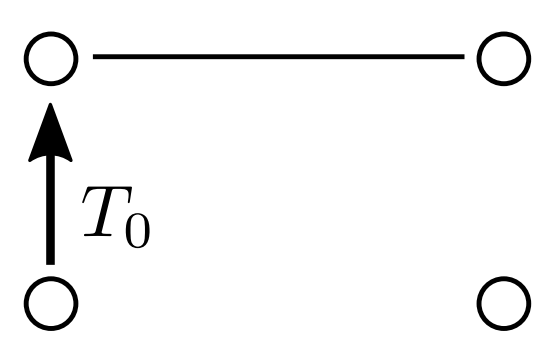
\includegraphics[width=0.2\linewidth]{images/gen.png}
    \caption{For two segments, $T_0$ represents the waiting time for the generation of a single link between two nodes without any intermediate repeater nodes.}
    \label{fig:gen}
\end{figure}


\subsection*{Werner Parameter for Elementary Entanglement}
... % TODO

\section*{Entanglement Swapping}

Once we have generated elementary entanglement, we can use it to \textbf{create entanglement over longer distances by entanglement swapping}.
We defined $T_0$ as the waiting time for the generation of elementary entanglement, and our base for the induction.
We now define our inductive step assuming that we have found an expression for $T_n$ and we want to construct $T_{n+1}$. 

In order to perform the entanglement swap to produce a single $(2^n+1)$-hop link, a node needs to wait for the production of two $(2^n)$-hop links, one on each side. 

Denote the waiting time for the pairs by $T_n^{(A)}$ and $T_n^{(B)}$, both of which are i.i.d. with $T_n$, as they are \hyperref[paragraph:copies_of_a_random_variable]{copies} of it. 

\subsubsection*{Time until both pairs are available}

We introduce a new random variable $M_n$ modeling the time until both pairs are available
\begin{equation}
    M_n := \max(T_n^{(A)} , T_n^{(B)})
\end{equation}
which is also \textbf{the time at which the entanglement swap ends}. 

This is distributed according to the CDF
\begin{equation}
    \Pr(M_n \leq t) = \Pr(T_n^{(A)} \leq t \text{ and } T_n^{(B)} \leq t) = \Pr(T_n \leq t) ^ 2.
\end{equation}

From it, we can derive the PDF
\begin{align}\label{eq:pdf_waiting_time_pair}
    \Pr(M_n = t) &= \sum_{\substack{t_A, t_B: \\ t = \max(t_A, t_B)}} \Pr(T_n^{(A)} = t_A \text{ and } T_n^{(B)} = t_B) .
\end{align}

% todo: add a concrete example coming from the code, with \Pr(T_n^{(A)} = t_A), \Pr(T_n^{(B)} = t_B and \Pr(M_n = t)

\subsubsection*{Number of steps required}

We introduce now $K_n$, a random variable following a \hyperref[subsection:geometric_pdf]{geometric distribution}
\begin{equation}
    \Pr(K_n = k) = p_{swap} (1 - p_{swap})^{k-1}
\end{equation}
modeling \textbf{the number of steps $k$ until the first successful swap} at level $n$.

The fact that it follows a geometric distribution is a direct consequence of our choice to model the success probability $p_{swap}$ to be independent of the state of the two input links. 

\subsubsection*{Derivation of $T_{n+1}$}
The derivation of $T_{n+1}$ requires us to combine the random variable for the number of steps required $K_n$ and the random variable for the waiting time for one attempt $M_n$.

In order to find the relation between $M_n$ and $T_{n+1}$, note that when entanglement swap fails, the two input are lost and need to be
regenerated. The regeneration of fresh entanglement after each failing entanglement swap adds to the waiting time. 

Thus, $T_{n+1}$ is a \textit{compound random variable}: it is the sum of $K_n$ copies of $M_n$. 

Since the number of entanglement swaps $K_n$ is geometrically distributed, we say that $T_{n+1}$ is a \textit{geometric compound sum} of $K_n$ copies of $M_n$, denoted as
\begin{equation}
    T_{n+1}=\sum_{k=1}^{K_{n}} M_{n}^{(k)}
\end{equation}

\subsubsection*{Derivation of the PDF of $T_{n+1}$}

The probability distribution of the waiting time $T_{n+1}$
\begin{align}
    \Pr(T_{n+1} = t) &= \Pr\left[\sum_{k=1}^{K_{n}} M_{n}^{(k)} = t\right] \\
    \intertext{is computed as the marginal of the waiting time conditioned on a fixed number of swaps}
    &= \sum_{k=1}^{\infty} \Pr(K_{n} = k) \cdot \Pr\left[\left( \sum_{j=1}^{k} M_{n}^{(j)} \right) = t\right].
\end{align}

We know $K_n$ is a geometric distribution and we know that the sum of probability distributions is the convolution.

Therefore, we can factor the constant out and get
\begin{equation}
    \Pr(T_{n+1} = t) = \sum_{k=1}^{\infty} p_{\text{swap}}(1 - p_{\text{swap}})^{k-1} \left( \ast_{j=1}^{k} m \right)
\end{equation}
where
\begin{equation*}
    m(t) := \Pr(M = t) = \sum_{\substack{t_A, t_B: \\ t = \max(t_A, t_B)}} \Pr(T_n^{(A)} = t_A \text{ and } T_n^{(B)} = t_B)
\end{equation*}
directly from \hyperref[eq:pdf_waiting_time_pair]{(29)}

\end{document}